\documentclass[a4paper,10pt]{article}
\usepackage[margin=1in, paperwidth=8.5in, paperheight=11in]{geometry}
\usepackage{amsfonts}
\usepackage{amssymb}
\usepackage[T1]{fontenc}
\usepackage{fancyvrb}
\usepackage[utf8]{inputenc}
\usepackage[english, italian]{babel}
\usepackage{tabularx}
\inputencoding{utf8}
\usepackage{float}
\usepackage{fancyhdr}
\usepackage{graphicx}
\pagestyle{fancy}
\renewcommand{\topfraction}{.9}
\renewcommand{\bottomfraction}{.9}
\renewcommand{\textfraction}{.1}
\fancyhf{}
\lfoot{Qontainer - Elisabetta Piombin - 1142189}
\pagestyle{plain}

\begin{document}
\title {Qontainer}
\author {Elisabetta Piombin 1142189}
\date{}

\maketitle
\tableofcontents
\clearpage\mbox{}

\section{Abstract}
\textbf{Qontainer} è un progetto realizzato al fine di fornire un contenitore che gestisca una libreria di contenuti multimediali: file audio e file video, che si dividono a loro volta in canzoni, podcast, serie tv e film. \\
Per farlo, la classe templatizzata \texttt{container} a sua volta fa uso di altre classi annidate:
\begin{enumerate}
\item \texttt{nodo}: inserita nella parte privata di \texttt{container}, viene usata per memorizzare i vari contenuti multimediali, visti come se fossero una lista concatenata di elementi, con ogni nodo diviso nel suo campo \texttt{info} (di tipo parametrico \texttt{T}, \texttt{next} e \texttt{prev} (di tipo \texttt{nodo*}). In \texttt{container} è presente un puntatore al primo elemento della lista.
\item \texttt{const\_iterator}: inserita nella parte pubblica di \texttt{container}, è la classe che permette l'implementazione di iteratori costanti.
\item \texttt{iterator}: inserita nella parte pubblica di \texttt{container}, è la classe che permette l'implementazione di iteratori non costanti.
\end{enumerate}
Vista l'assenza di puntatori ad altre classi nella gerarchia, è stata ritenuta superflua l'implementazione di una classe per un eventuale \textit{smart pointer}.\\
Ho scelto di implementare il contenitore come una lista doppiamente linkata composta da nodi perché offro la possibilità di rimuovere contenuti all'interno della libreria in posizioni arbitrarie, e questo mi porta alla necessità di scegliere l'implementazione sotto forma di lista, che rende tale operazione di rimozione più efficiente (viene operata in tempo costante) rispetto alla scelta di implementare tale contenitore come un vettore di elementi.
\section{Manuale utente}
In questa sezione vengono descritte le varie schermate della GUI.\\
\subsection{Finestra principale}

\begin{figure}[H]
	\begin{center}
		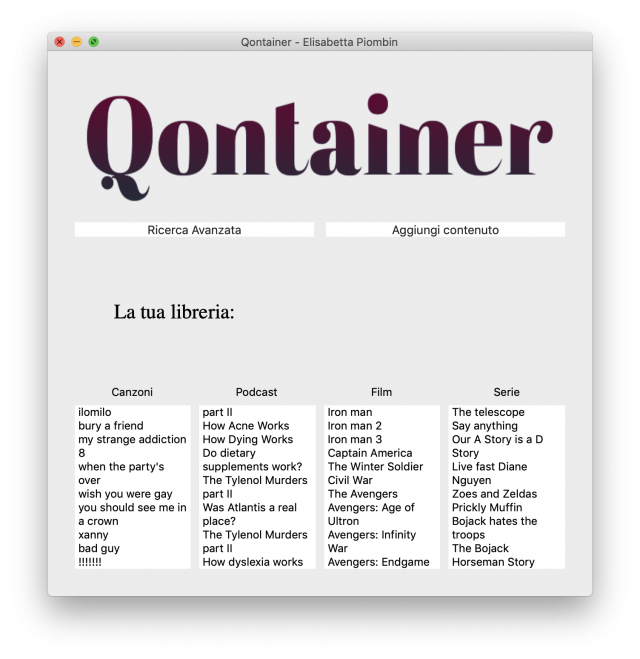
\includegraphics[width=\textwidth,keepaspectratio]{immagini/MainWindow.png}
	\end{center}
	\caption{\label{fig:my-label} Finestra principale del progetto}
\end{figure} 

Da qui si ha un'\textit{overview} dell'intera applicazione, con tutti i contenuti in essa inseriti dall'utente, suddivisi per \textbf{Canzoni}, \textbf{Podcast}, \textbf{Film} e \textbf{Serie}. Tramite la finestra principale si da' all'utente la possibilit\`a di cercare o di aggiungere contenuto.\\
\subsection{Aggiunta di contenuto}
\begin{figure}[H]
	\begin{center}
		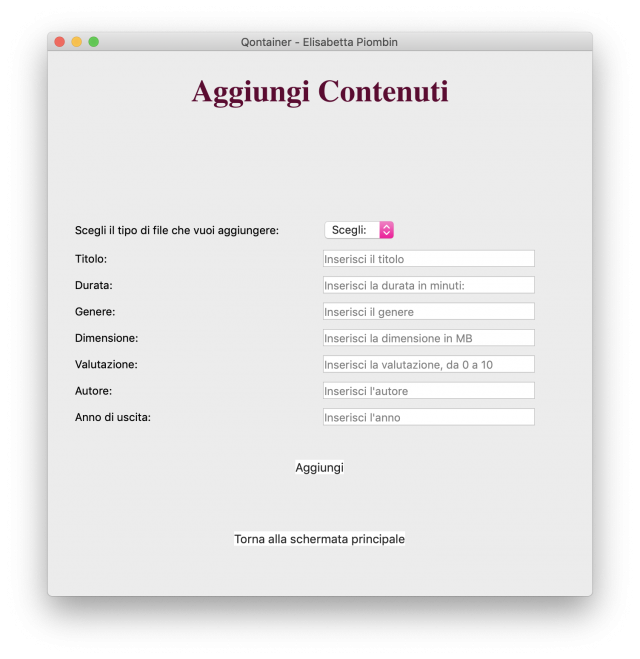
\includegraphics[width=\textwidth,keepaspectratio]{immagini/AggiungiContenuti.png}
	\end{center}
	\caption{\label{fig:my-label} Finestra base di aggiunta contenuti}
\end{figure}
\begin{figure}[H]
	\begin{center}
		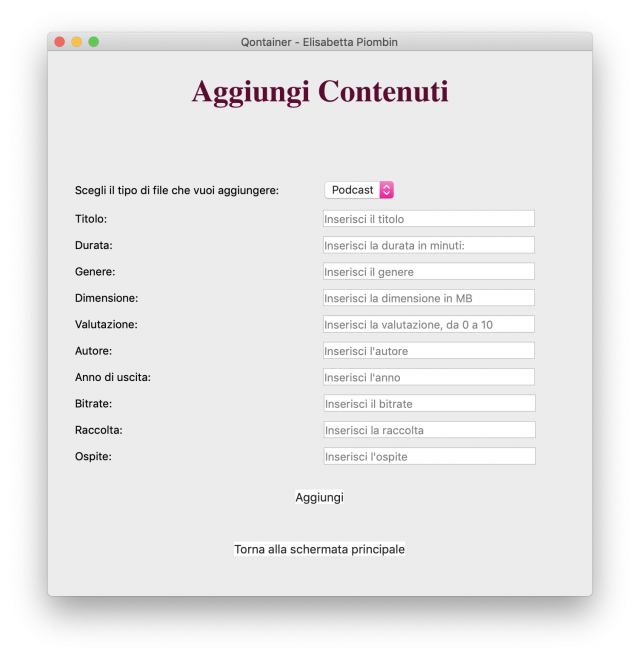
\includegraphics[width=\textwidth,keepaspectratio]{immagini/AggiungiContenuti2.png}
	\end{center}
	\caption{\label{fig:my-label} Finestra specifica di aggiunta contenuti}
\end{figure}
Nella schermata di aggiunta dei contenuti l'utente deve scegliere il tipo di contenuto che vuolei inserire, e a seconda della scelta compariranno i campi dati specifici di quella classe. Ad esempio, nella \textit{Figura 3} è stato scelto di inserire un podcast, e questo ha fatto comparire i campi \textit{Bitrate, Raccolta} e \textit{Ospite}. \\
Dopo aver schiacciato il bottone \textit{Aggiungi}, l'utente si trova una finestra di conferma di aggiunta riuscita.

\subsection{Ricerca del Contenuto}
\begin{figure}[H]
	\begin{center}
		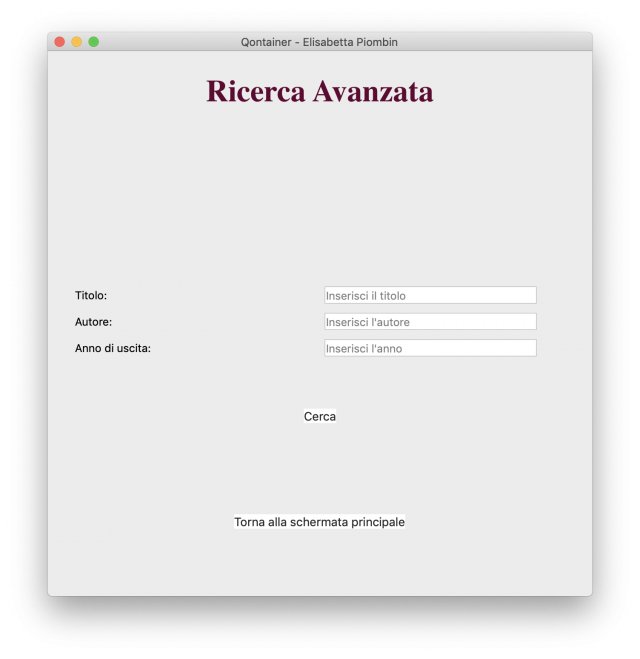
\includegraphics[width=\textwidth,keepaspectratio]{immagini/RicercaAvanzata.png}
	\end{center}
	\caption{\label{fig:my-label} Prima finestra di ricerca}
\end{figure}
All'utente viene data la possibilit\`a di modificare i contenuti esistenti, e la ricerca per la modifica \`e implementata in modo che accetti sia stringhe incomplete che \textit{upper} o \textit{lower case}. All'utente viene data solamente la possibilit\`a di inserire i campi dati che \`e pi\`u probabile vengano ricordati a memoria, per avere una ricerca realistica: sarebbe impossibile che l'utente si ricordi il valore di ogni singolo campo dato di ogni oggetto inserito nell'applicazione.\\
Una volta inserito anche solo un campo dato parziale (nell'esempio ho inserito solamente "iron" nel campo del titolo), l'utente si vede restituire tutti i match trovati all'interno dell'applicazione:
\begin{figure}[H]
	\begin{center}
		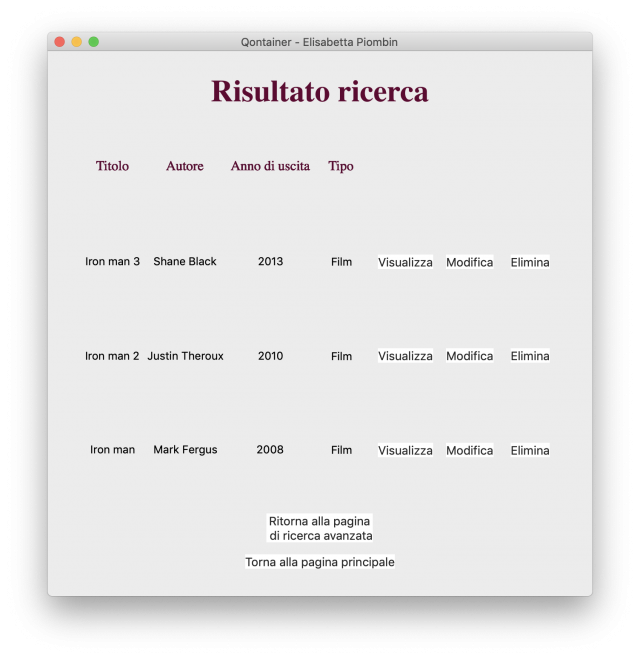
\includegraphics[width=\textwidth,keepaspectratio]{immagini/RisultatoRicerca.png}
	\end{center}
	\caption{\label{fig:my-label} Risultato della ricerca}
\end{figure}
\noindent
Una volta aperta la finestra dei risultati, all'utente viene data la possibilit\`a di \textbf{visualizzare} nel dettaglio, \textbf{modificare} oppure \textbf{eliminare} del contenuto.
\begin{figure}[H]
	\begin{center}
		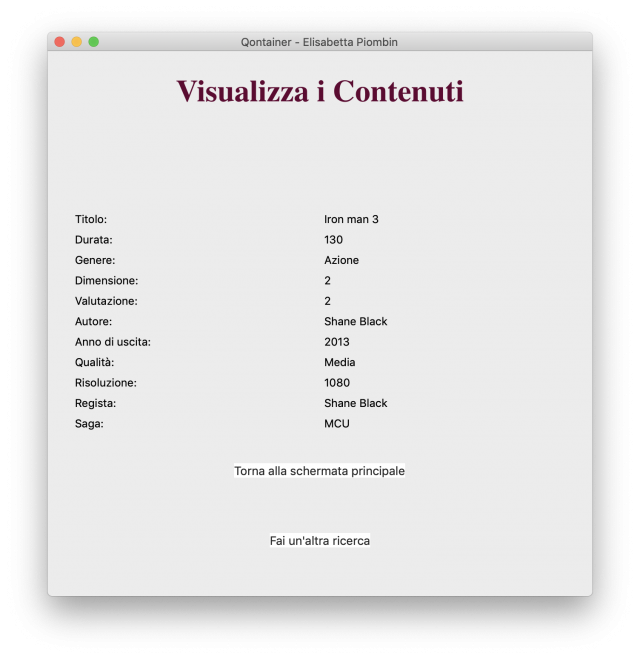
\includegraphics[width=\textwidth,keepaspectratio]{immagini/VisualizzaContenuti.png}
	\end{center}
	\caption{\label{fig:my-label} Visualizzazione dettaglio contenuti}
\end{figure}

\begin{figure}[H]
	\begin{center}
		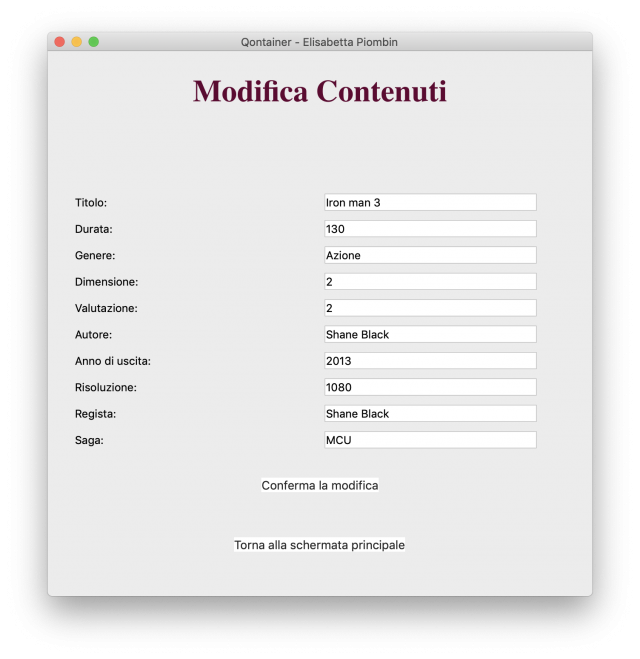
\includegraphics[width=\textwidth,keepaspectratio]{immagini/ModificaContenuti.png}
	\end{center}
	\caption{\label{fig:my-label} Modifica dei contenuti}
\end{figure}
\section{Compilazione ed esecuzione}
La compilazione si esegue tramite i comandi \texttt{qmake} e in seguito \texttt{make}. 

\section{Descrizione della gerarchia di classi}

La classe base astratta da cui deriva tutta la gerarchia è \texttt{ContenutoMultimediale}, che verrà poi concretizzata tramite sue classi derivate.
Da \texttt{ContenutoMultimediale} derivano immediatamente altre due classi: \texttt{audio} e \texttt{video}, che sono le due macrocategorie di appartenenza dei file che vengono memorizzati nella libreria. \\
Da \texttt{video} derivano due classi: \texttt{film} e \texttt{episodio}, mentre da \texttt{audio} derivano altre due classi, \texttt{podcast} e \texttt{canzone}. \\
Non si verifica la situazione di ereditarità multipla. \\
\begin{figure}[H]
	\begin{center}
		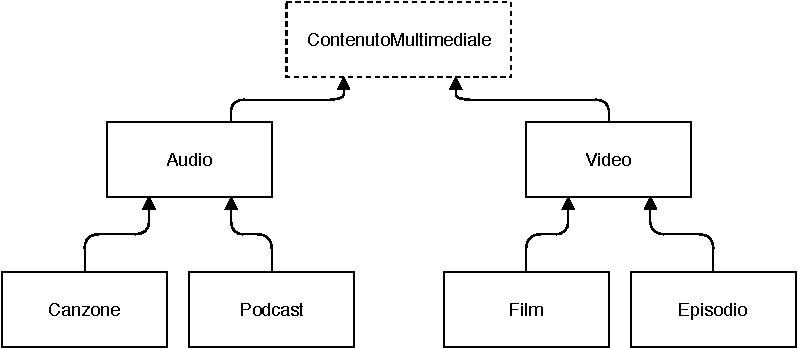
\includegraphics[width=\textwidth,keepaspectratio]{immagini/classi.pdf}
	\end{center}
	\caption{\label{fig:my-label} Gerarchia delle classi}
\end{figure}



\section{Descrizione delle chiamate polimorfe}
Sono presenti tre metodi virtuali nella gerarchia: \texttt{serializza(char)}, l'overloading dell'operatore di confronto \texttt{operator==(const T\&)}, e il metodo \texttt{qualita()}, che è puro.
\begin{enumerate}
	\item [-] \texttt{string serializza(char)}: definito virtuale all'interno di \texttt{ContenutoMultimediale}, viene implementato diversamente per i campi dati specifici di ogni classe derivata. Viene richiamata all'interno della classe \texttt{database}, all'interno della funzione \texttt{void save(container<T>\&)}, in quanto questa è la funzione che si occupa del salvataggio su file degli oggetti inseriti dentro al \texttt{container}.
	\item [-] \texttt{bool operator== (const T\&)} è usato nella funzione \texttt{void remove(T)} all'interno di \texttt{ContenutoMultimediale}, e viene usata in \texttt{risultatoricerca} (nella GUI) per rimuovere un elemento dal contenitore. L'operatore di uguaglianza non viene usato nell'operazione di ricerca, nonostante potrebbe sembrare immediato il suo utilizzo in tale contesto. Per la ricerca dei contenuti all'interno del \textit{container} ho implementato una funzione \texttt{vector<T> search (T)}.
	\item [-] \texttt{string qualita() const}, metodo virtuale puro in \texttt{ContenutoMultimediale}, utilizzato in \texttt{visualizzaelemento} per dare la possibilità all'utente per vedere se il file che si sta visualizzando è di qualità media, alta o bassa. Ha diverse implementazioni in \texttt{audio} e in \texttt{video}.
\end{enumerate}
Nella classe base \texttt{ContenutoMultimediale} è presente il distruttore virtuale di default.



\section{Descrizione del formato del file di salvataggio e caricamento del contenitore}
Per il caricamento dei file che compongono la libreria, e per il loro salvataggio, mi appoggio ad una classe esterna alla gerarchia, che ho chiamato \texttt{database}. Questa classe contiene i metodi \texttt{load()} e \texttt{save()}. La classe \texttt{database} non è un template perché dipende strettamente da \texttt{ContenutoMultimediale}. 
\begin{enumerate}
\item[-] \texttt{void load(container<ContenutoMultimediale*>\&)}, tramite un'operazione di deserializzazione implementata ad hoc in ogni classe derivata concreta della gerarchia, permette la lettura del contenuto in ogni file \texttt{.txt}. Esiste un unico file \texttt{.txt}, in cui sono scritti tutti gli oggetti che verranno caricati nel \texttt{container}.  Database si occupa di caricare questi oggetti nella libreria tramite:
\begin{enumerate}
	\item \texttt{static film* film::deserializza(const vector<string>\&)}
	\item \texttt{static episodio* episodio::deserializza(const vector<string>\&)}
	\item \texttt{static podcast* podcast::deserializza(const vector<string>\&)}
	\item \texttt{static canzone* canzone::deserializza(const vector<string>\&)}
\end{enumerate} 
In modo che possano essere gestiti dal contenitore templetizzato.
\item[-] \texttt{void save(container<ContenutoMultimediale*>\&)} si occupa di memorizzare sul file \texttt{.txt} i caratteri corrispondenti agli oggetti contenuti in \texttt{container}, invocando polimorficamente il metodo \texttt{serializza(char)} corretto, che è definito come virtuale.
\end{enumerate}

\section{Tempistiche}

\begin{center}
 \begin{tabular}{||c | c ||} 
 	\hline
 \hline
 \textbf{Ore} & \textbf{Fase}  \\ 
 \hline\hline
 2 & Analisi preliminare del problema \\ 
 \hline
 1 & Progettazione del modello \\
 \hline
 1 & Progettazione della GUI\\
 \hline
 10 & Apprendimento libreria Qt \\
 \hline
 30 & Codifica modello e GUI\\ 
 \hline
 10 & Debugging \\
 \hline
 5 & Testing\\
 \hline
 \hline
\end{tabular}
\end{center}

\end{document}